\chapter{Introducción}
\label{chap:introduccion}

%%%%%%%%%%%%%%%%%%%%%%%%%%%%%%%%%%%%%%%%%%%%%%%%%%%%%%%%%%%%%%%%%%%%%%%%%%%%%%%%
% Objetivo: Exponer de qué va este proyecto, sus líneas maestras, objetivos,   %
%           etc.                                                               %
%%%%%%%%%%%%%%%%%%%%%%%%%%%%%%%%%%%%%%%%%%%%%%%%%%%%%%%%%%%%%%%%%%%%%%%%%%%%%%%%


\section{Motivación} 
 \label{sec:intro-motivation}
 
 %En el punto 1.1 debes poner algo así (escrito por mi, lo puedes usar):
El Grupo Integrado de Ingeniería (GII) de la Universidade da Coruña (UDC) viene desarrollando una línea de investigación en Robótica y Cognición desde hace más de 15 años, que tiene como objetivo general desarrollar sistemas reales que puedan responder con el mayor grado de autonomía posible a las condiciones cambiantes del medio, sin tener que precisar de la ayuda de un operador o programador para establecer las nuevas estrategias necesarias para la consecución de la tarea encomendada. Esta línea de investigación tiene otra línea derivada que se denomina Mecanismos Cognitivos, en la cual se centra en el estudio e implementación de funcionalidades cognitivas de alto nivel en robots autónomos, utilizando los procesos cognitivos humanos como inspiración para desarrollar un mecanismo cognitivo completo para un robot. 
Uno de los proyectos asociados a la línea de Mecanismos Cognitivos es DREAM\cite{dream_project} (Deferred Restructuring of Experience in Autonomous Machines), financiado por la Unión Europea, y que se centra en la integración de procesos cognitivos basados en el sueño dentro de una arquitectura cognitiva para robots autónomos. El objetivo de utilizar estos procesos reside en la capacidad de consolidar el aprendizaje adquirido durante la operación en "tiempo de vida" que se ha visto que existe en los procesos asociados al sueño en el cerebro humano. De esta forma, la experiencia adquirida por el robot se analiza y procesa en otra escala temporal que proporciona nuevas representaciones de más alto nivel. 
Uno de los principales problemas a solucionar en el proyecto DREAM se centra en el aprendizaje a partir de la interacción con humanos. En este sentido, se requieren numerosos datos de interacción en tiempo real en diversas situaciones para poder mejorar la arquitectura, y para lograrlos se ha diseñado la iniciativa \enquote{adopt a robot}. Esta iniciativa se centra en proporcionar a los centros educativos un robot de bajo coste que contenga la arquitectura cognitiva desarrollada en el DREAM, de modo que los alumnos puedan interactuar con el robot libremente y se consiga gran variedad de datos para mejorar dicha arquitectura. Este robot está en desarrollo actualmente en el GII bajo el nombre de ROBOBO, y es en el que se centrará el presente TFG.
 El ROBOBO se basa en el uso de una plataforma motorizada y sensorizada, llamada ROB en el sistema, que se conecta a un Smartphone, llamado OBO, que se encarga del procesado de los datos recogidos desde la plataforma y de controlar las acciones de la misma. Este tipo de arquitectura presenta numerosas ventajas que resultaron interesantes a la hora de escogerlo para su uso en DREAM:
 \begin{itemize}
 	\item Bajo coste de la plataforma
 	\item Gran capacidad de sensorización, cualquier smartphone de gama media cuenta con acelerómetros, giroscopios, gps, cámara y micrófono, y de comunicaciones, wifi, gsm y bluetooth.
 	\item Robot fácilmente actualizable, mediante el cambio de smartphone, sin necesidad de adaptar el software antiguo.
 	\item Gran disponibilidad de smartphones, todos los usuarios potenciales poseen uno, además Android, sistema operativo escogido para el sistema, cuenta con un 82.8\% de la cuota de mercado.
 \end{itemize}
%A continuación deberías poner lo que tienes ahora mismo en el punto 2.2 sobre el ROBOBO 1.0 y el 2.0, ligándolo con lo anterior. Es decir, explica que se desarrolló una primera versión del ROBOBO y ahora se está en otra más avanzada. 

\subsection{Robobo 1.0}
\begin{figure}
	\centering
	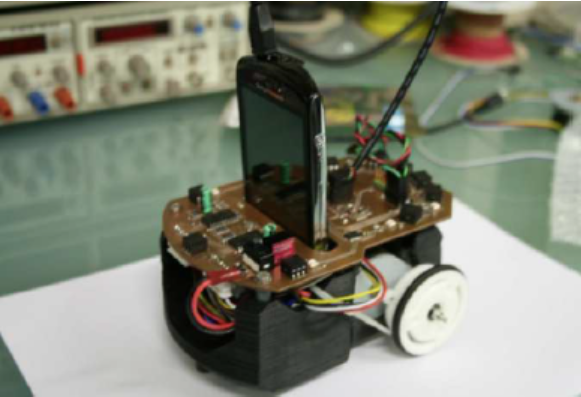
\includegraphics[width=0.8\linewidth]{imagenes/robobo1_0.PNG}
	\caption{Robobo 1.0}
	\label{fig:robobo_1_0}
\end{figure}

La primera versión de la plataforma  desarrollada por el GII fue el ROBOBO 1.0 (Figura \ref{fig:robobo_1_0}), que sirvió como versión conceptual para comprobar la viabilidad del sistema plataforma + smartphone, y presentaba las siguientes características:

\begin{itemize}

	\item 9 LEDs (diodos emisores de luz) RGB para interactuar con el usuario, que cambiaban de color con la proximidad de objetos.
	\item 9 sensores IR de proximidad para proporcionar capacidad de movimiento autónomo: 2 en la parte frontal, 4 en los laterales y los últimos tres en la parte trasera; de manera que proporcionaba una visión general del entorno.
	\item 2 motores paso a paso (convierten impulsos eléctricos en desplazamientos angulares discretos, es decir, pueden avanzar un ángulo concreto en función de la señal recibida) que aplicaban movimiento a las ruedas, con un paso de 1/8, con gran precisión de giro.
	\item Compatibilidad con dispositivos Android.
	\item Capacidad de interacción con otros dispositivos ROS.
	\item Conexión USB para la comunicación con el teléfono inteligente.

\end{itemize}

\subsection{Robobo 2.0}
\begin{figure}
	\centering
	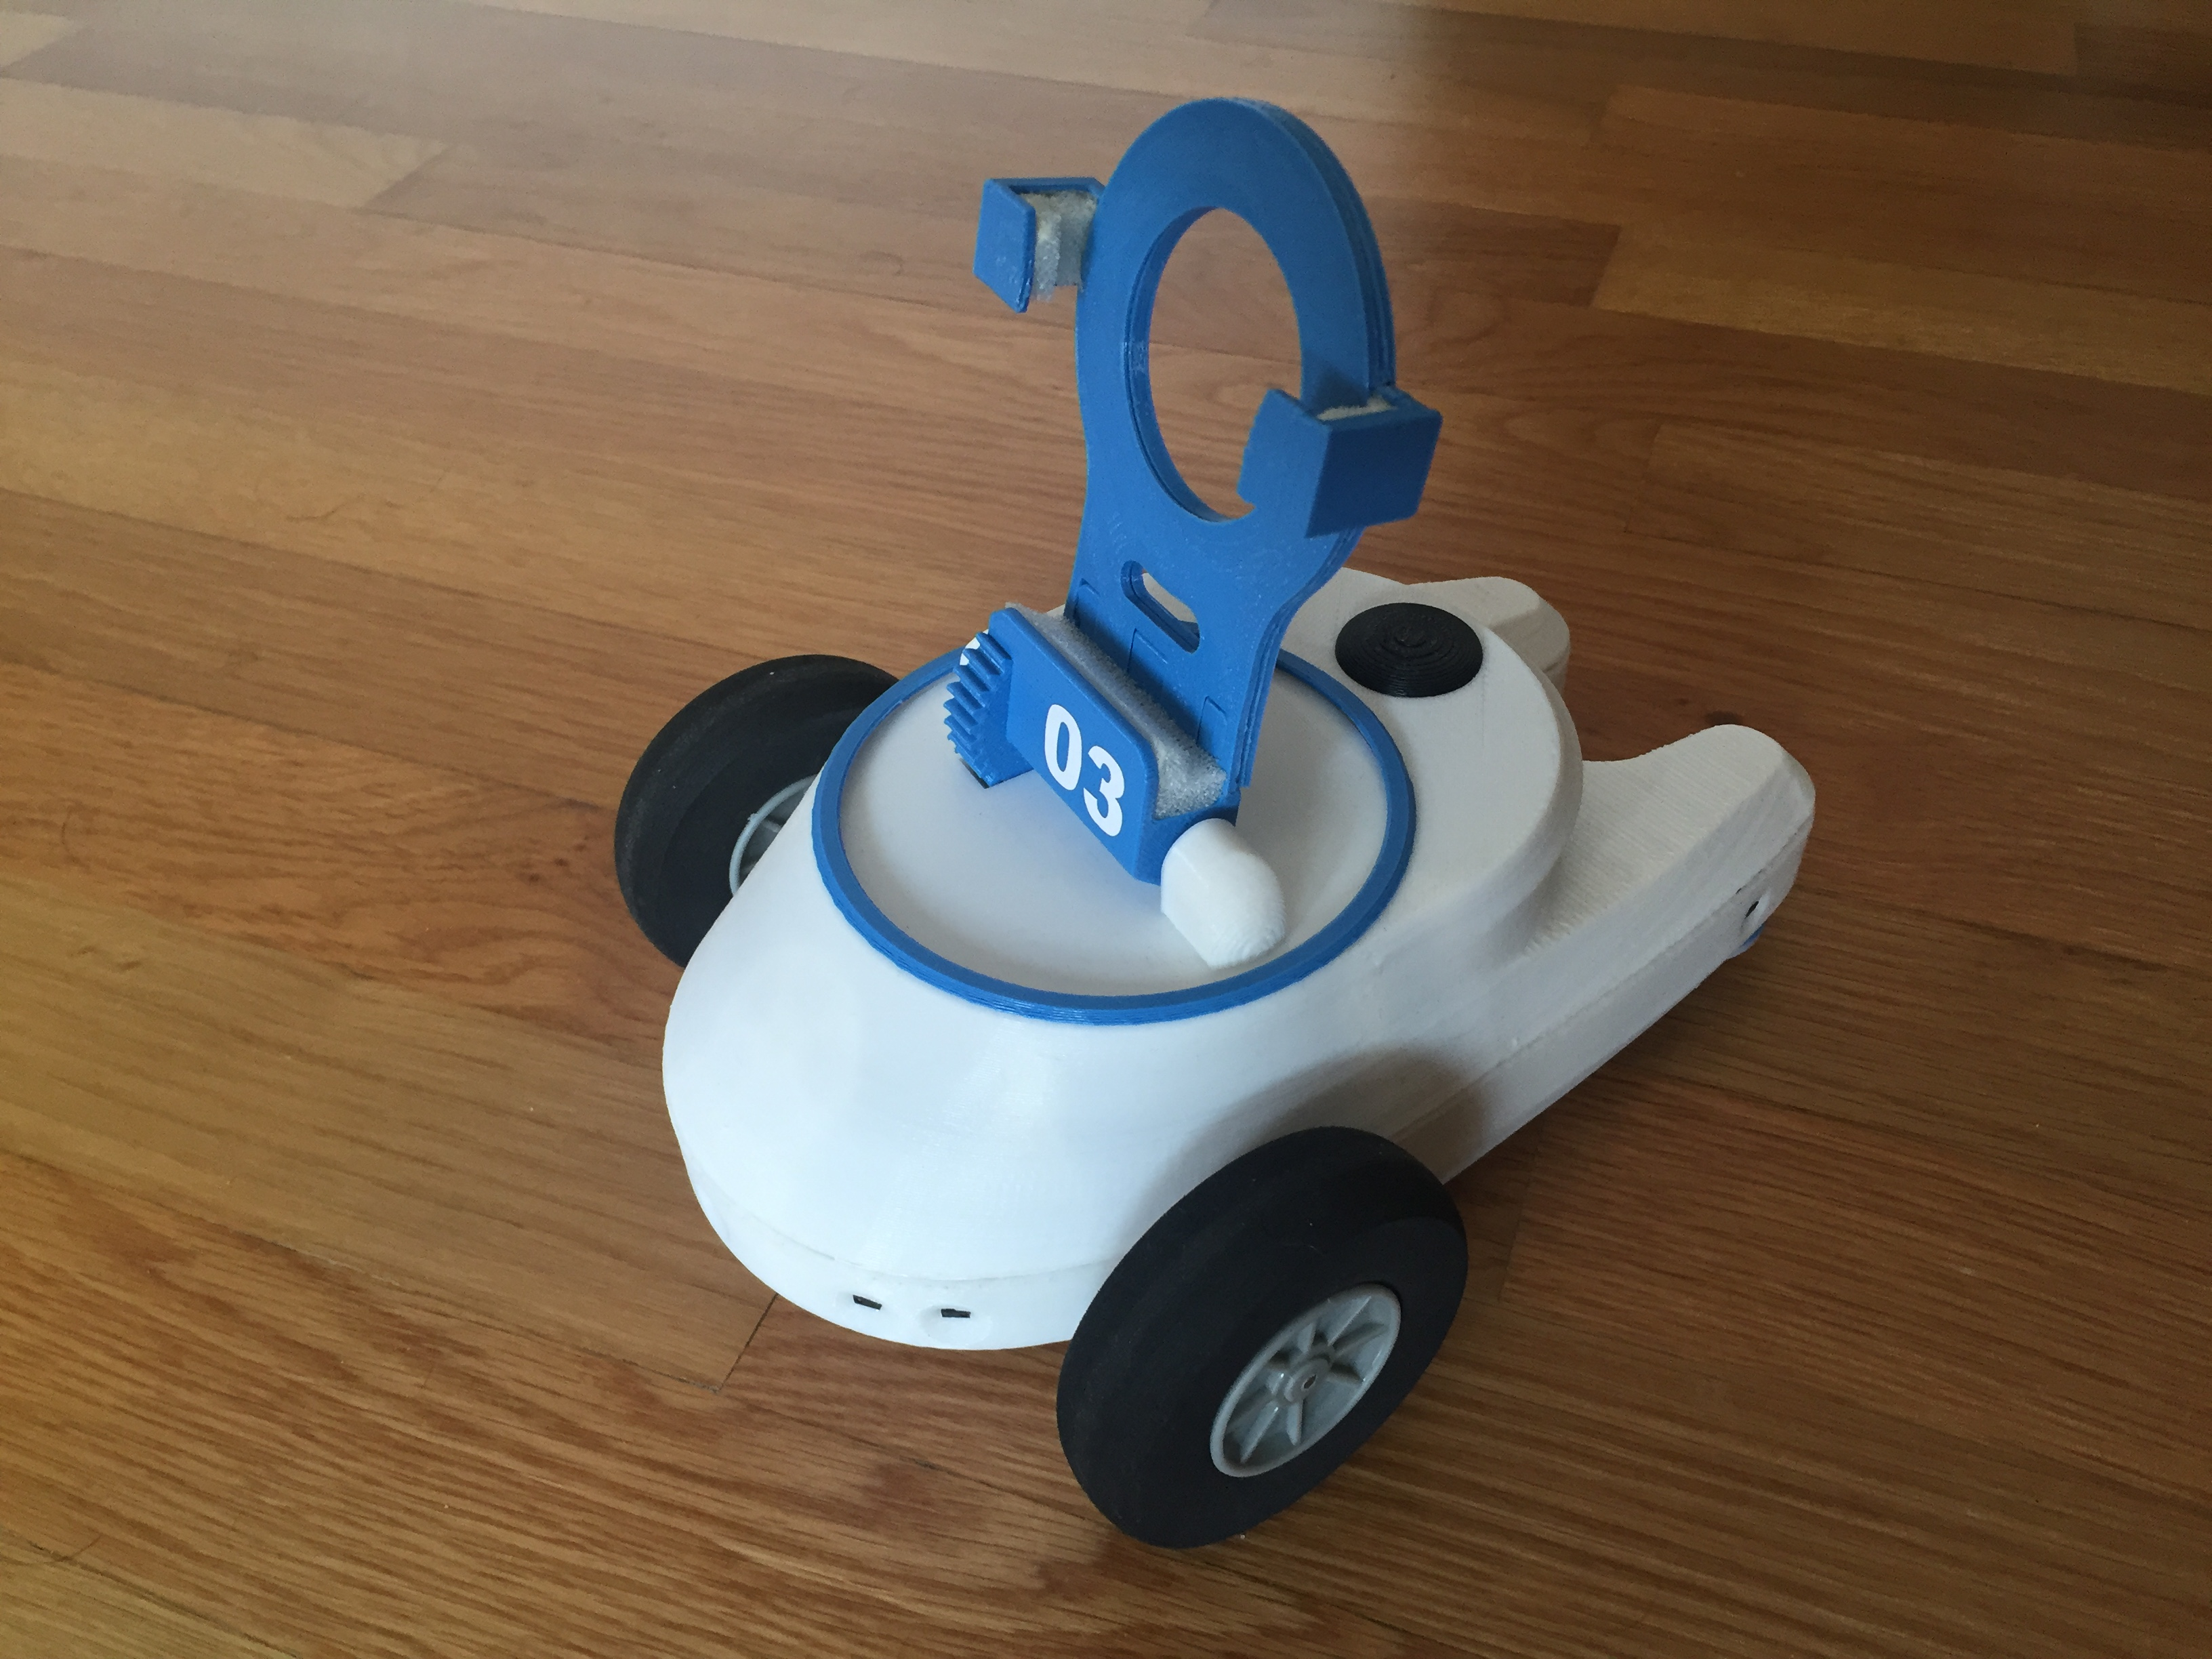
\includegraphics[width=0.8\linewidth]{imagenes/robobo_rob.JPG}
	\caption{Robobo 2.0}
	\label{fig:robobo_2_0}
\end{figure} 

La segunda versión, el ROBOBO 2.0 (figura \ref{fig:robobo_2_0}), trata de solventar las carencias de la primera versión y añadir ciertas mejoras. Tras este rediseño, las características del robot pasaron a ser:

\begin{itemize}	
%todo los leds son 9?

	\item LEDs: pasan a ser 21, 9 de ellos formando una matriz de comunicación para dar una información avanzada mediante colores y formas.
	\item Motores de las ruedas: Pasan a ser motores de corriente continua, menos voluminosos y más eficientes energéticamente. Cada motor cuenta con un encoder magnético, que transforma el movimiento del motor en pulsos eléctricos, que pueden ser interpretados por la parte software del robot.
	\item Comunicación: Se elimina la comunicación USB a favor de una conexión Bluetooth, lo cual permite utilizar diferentes smartphones con distintas posiciones de los puertos.
	\item Plataforma universal para smartphones: Se incluye un adaptador universal para teléfonos móviles, montado sobre una plataforma motorizada que permite el movimiento del smartphone sobre el chasis del robot. Esta plataforma tiene dos grados de libertad, rotación e inclinación.
	\item Sensores: Modificadas tanto el tipo, la cantidad y la posición. Se colocaron en la siguiente disposición (figura \ref{fig:robobo_2_0_sensors}):
	\begin{figure}
	\centering
	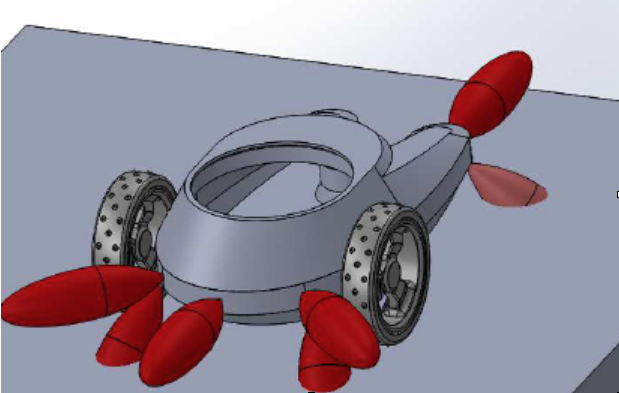
\includegraphics[width=0.8\linewidth]{imagenes/robobo_2_sensors.png}
	\caption{Disposición de los sensores en el ROBOBO 2.0}
	\label{fig:robobo_2_0_sensors}
\end{figure} 
	\begin{itemize}
	\item 3 sensores para la detección de colisiones en la parte delantera; uno frontal y los otros dos cercanos a las ruedas, de tal forma que el ROBOBO no pudiera chocar, frontalmente con ninguna superficie.
	\item 2 sensores inclinados hacia abajo para la detección de caídas, en la parte delantera, colocados cerca de las ruedas, es decir, la zona con mayor peligro de caídas.
	\item 2 sensores de caídas y 2 de colisiones, de forma similar a los anteriores, en la zona anterior del robot. 
	
	\end{itemize}
	\item Unión sensores-microcontrolador: se han cambiado las resistencias pull-up anteriores por un multiplexor. Se consigue, así, un único elemento de muchas entradas y una única salida capaz de permitir la transmisión de una, y solo una, de las entradas hacia la salida.

	\item Microcontrolador: PIC32MX534F064H, de la familia de microcontroladores de 32 bits, económico, con alta capacidad de procesamiento, diversidad de interfaces de comunicación y multitud de puertos de entrada y salida; además de que su entorno de desarrollo y su compilador son gratuitos. Este microcontrolador se programa mediante el protocolo de comunicación I2C y logra el contacto entre sensores y microcontrolador mediante buses línea de reloj “SCL” y buses línea de datos “SDA”.




\end{itemize}

Esta versión del ROBOBO, aún en pleno desarrollo, es la que se utilizará en este trabajo de final de grado que se centrará en el desarrollo de  librerías de interacción básica entre el robot y humanos, enfocándose específicamente en interacción por voz, táctil, sonido e imagen, dando lugar a módulos simples que más tarde podrán se combinados en comportamientos interactivos más complejos. El desarrollo fundamental de este trabajo se realizará en Android, ya que inicialmente el ROBOBO solo soportará teléfonos con este sistema operativo. 

%Para terminar este punto 1.1 de Motivación, deberías comentar que la versión 2.0 está en pleno desarrollo y poner algo parecido a lo que pusimos en el anteproyecto:
%En este trabajo Fin de Grado se deberán implementar diversas librerías de interacción básica del robot con humanos, centradas fundamentalmente en interacción por voz, imagen y gestos con el smartphone. El desarrollo fundamental de este trabajo se realizará en Android, ya que inicialmente el ROBOBO solo soportará teléfonos con este sistema operativo. Se comenzará por desarrollar módulos de interacción simples que más tarde serán combinados para dar lugar a comportamientos interactivos más complejos.
%Durante el desarrollo de estas librerías podrá ser necesaria la interacción con el software de control de bajo nivel de la plataforma, de modo que se ajuste este a los requerimientos de los comportamientos más complejos.

 \section{Objetivos}
 \label{sec:intro-objetives}
 El objetivo de este proyecto, como se comentó en la sección anterior, es el desarrollo de librerías que permitan una interacción básica entre el ROBOBO y humanos. Estas librerías serán desarrolladas en Android, sistema operativo que soporta el ROBOBO a día de hoy. Se desarrollarán 5 librerías Android, cada una enfocada a un tipo de interacción diferente con el robot:
 \begin{itemize}
 	\item Librería de interacción por voz
 	\item Librería de interacción por sonido
 	\item Librería de interacción táctil
 	\item Librería de interacción por imagen
 	\item Librería de interacción mediante mensajes
 \end{itemize} 
 Finalmente se implementarán una serie de ejemplos para demostrar el funcionamiento de las diferentes librerías de forma conjunta.
  %A continuación vendría el apartado 1.2 donde pones el objetivo global y los sub-objetivos en que se divide
 \section{Estructura de la memoria}
 \label{sec:intro-memory-structure}
 La memoria del trabajo está estructurada en 6 capítulos, siendo el primero de ellos esta introducción.
 \begin{itemize}
 	\item Segundo capítulo: \textbf{\textit{Fundamentos teóricos}}, se habla sobre el ROBOBO! Framework, marco de desarrollo empleado para el desarrollo de los módulos que componen este trabajo, cómo interactúa con las diferentes partes del sistema ROBOBO y las tecnologías en las que se basa.
 	
 	\item Tercer capítulo: \textbf{\textit{Antecedentes}}, se hablará sobre el campo de la interacción humano robot y se expondrán ejemplos de los diferentes modos de interacción que surgen en los diferentes campos de la robótica. 
 	\item Cuarto capítulo: \textbf{\textit{Fundamentos Tecnológicos}} se dará un repaso a las diferentes tecnologías empleadas a la hora del desarrollo de los módulos de interacción.
 	
 	\item Quinto capítulo: \textbf{\textit{Desarrollo}}, se elabora el desarrollo técnico del trabajo, el modelo conceptual, la arquitectura escogida, la metodología seguida y los detalles de implementación. 
 	
 	\item Sexto capítulo: \textbf{\textit{Resultados y pruebas}}, se comentan los resultados del desarrollo y se exponen las aplicaciones de ejemplo desarrolladas utilizando los módulos de interacción. También se exponen los problemas conocidos aún sin solución.
 
 	\item Séptimo capítulo: \textbf{\textit{Conclusiones}}, en este último capítulo se comenta el resultado general del trabajo así como el trabajo futuro a desarrollar.


 \end{itemize}
 
 \section{Herramientas utilizadas}
  \label{sec:intro-tools}
 Para el desarrollo de las librerías y aplicaciones Android que conforman el presente trabajo, se ha empleado el entorno de desarrollo \textbf{Android Studio}, basado en el IntelliJ IDEA de Jetbrains. Actualmente Android Studio es el entorno de desarrollo oficial para Android.
 
 Para la creación de los diagramas se ha empleado el software \textbf{StarUML}.
 
 Para la redacción de la memoria se ha empleado el software \textbf{Texpad}.
 
 
 
  
 
 
 % Finalmente deberías hacer un apartado 1.3 donde comentas la estructura de la memoria, sobre todo del apartado de desarrollo y pruebas



